\section{Experimental Analyses}
\label{sec:experiments}

Our experiments were designed to validate the theoretical motivation for anchor points, evaluate VFMs on RSC, and analyze how different design choices affect rolling shutter correction and depth estimation quality. 

\subsection{Anchor Points for Controlled Synthetic Scenes}

We conduct single-scene experiments on the synthetic dataset \textbf{SYN1} to isolate the effect of anchor-point selection. Scenes exhibit rotation about the image center, suggesting an optimal anchor of $t_a=\frac{N}{2}$. Six diffusion models were trained across three scenes, comparing optimal ($t_a = \frac{N}{2}$) and suboptimal anchor points. Only models trained with the optimal anchor successfully corrected all three scenes, confirming our theoretical predictions (Fig.~\ref{fig:rotated_fig_sidepsnr}, Table \ref{table:AnchorPoint_single}). We further compare against Manhattan World~\cite{Manhattan} and RS-Diffusion~\cite{RS-Diffusion}, which struggle under extreme distortions.
% We begin with controlled single-scene experiments to isolate the effect of anchor point selection. Diffusion models were trained on individual scenes from the synthetic dataset \textbf{SYN1}, where the axis of rotation is fixed at the image center, suggesting an optimal anchor point of $t_a = \frac{N}{2}$.



% We further compared our pipeline with \textbf{Manhattan World}~\cite{Manhattan} and \textbf{RS-Diffusion}~\cite{RS-Diffusion}. These general-purpose methods struggle with the extreme distortions in SYN1, whereas our VFM pipeline preserves structure and continuity.
% \begin{table*}
%   \caption{Comparisons of different anchor points with the first stage of our two stage architecture. Three separate anchor points were tested $t_a = 0, \frac{N}{4}, \frac{N}{2}$. The models were run on the single scene datasets, the modified X4K dataset, and a subset of the real world collocated dataset. These comparisons were done on the intermediate RGB images, and $t_a = \frac{N}{2}$ outperforms all other anchor points. }
%   \centering
%   \begin{tabular}{c c c c cc c  c c  c c }
%     \hline
%        \multirow{2}{*}{Anchor} & \multicolumn{2}{c}{Ceiling Fan} & \multicolumn{2}{c}{Table Fan}& \multicolumn{2}{c}{Plane} & \multicolumn{2}{c}{X4K} & \multicolumn{2}{c}{Collocated}\\

%       &PSNR &SSIM&PSNR &SSIM&PSNR &SSIM & PSNR & SSIM & PSNR & SSIM \\
%     \hline
%       $t_a=0$& 34.93 & 0.971 & 26.82 & 0.831 & 24.21 & 0.808 &15.594 & 0.578 & 20.238 & 0.639\\
%       $t_a=\frac{N}{4}$&&&&&&&  17.291 & \textbf{0.630} & 20.292 & 0.640\\
%       $t_a=\frac{N}{2}$ & \textbf{36.21} & \textbf{0.986} & \textbf{27.57} & \textbf{0.842} & \textbf{25.02} & \textbf{0.841} & \textbf{17.733} & 0.629 & \textbf{21.778} & \textbf{0.674}\\



%     \hline
%     %3.66, 2.8, 3.35
%     %0.51, 1.32, 0.74
%   \end{tabular}

%   \label{table:AnchorPoint}
% \end{table*}

\begin{table}[th!]
  \caption{Comparisons of different anchor points with the first stage of our two-stage architecture on single-scene datasets (Ceiling Fan, Table Fan, Plane). The models were evaluated using PSNR and SSIM on intermediate RGB images. $t_a = \frac{N}{2}$ achieves the highest performance across all scenes.}
  \centering
  \setlength{\tabcolsep}{4pt} % tighten column spacing
  \begin{tabular}{c c c c c c c}
    \hline
    \multirow{2}{*}{Anchor} & \multicolumn{2}{c}{Ceiling Fan} & \multicolumn{2}{c}{Table Fan} & \multicolumn{2}{c}{Plane} \\
    & PSNR & SSIM & PSNR & SSIM & PSNR & SSIM \\
    \hline
    $t_a=0$ & 34.93 & 0.971 & 26.82 & 0.831 & 24.21 & 0.808 \\
    $t_a=\frac{N}{2}$ & \textbf{36.21} & \textbf{0.986} & \textbf{27.57} & \textbf{0.842} & \textbf{25.02} & \textbf{0.841} \\
    \hline
  \end{tabular}
  \label{table:AnchorPoint_single}
  % \vspace{-3mm}
\end{table}






% \begin{table*}[h]
%   \caption{Comparisons of PSNR, SSIM, AbsRel, and $\delta_1$ on the testing dataset used in Sect. 5.2. Our fine-tuned, two-stage architecture (U-Net, Transformer) performs better on validation than any other combination of the architectures. Values that are not possible to record (intermediate RGB metrics for one-stage architecture) are represented with NA.}
%   \centering
%   \begin{tabular}{c c  c c  c c  }
%     \hline
%       \multirow{2}{*}{Architecture} & \multirow{2}{*}{Method} &  \multicolumn{2}{c}{Intermediate RGB} & \multicolumn{2}{c}{Depth Map}\\
%      \cmidrule(lr){3-4} \cmidrule(lr){5-6} 
%       &&PSNR &SSIM  & AbsRel & $\delta_1$\\
%       \hline
%     \multirow{3}{*}{One Stage} & \cite{Marigold} & NA  & NA~ &6.047 &0.743\\
%     &\cite{DepthAnything}& NA &  NA & 0.655 & 0.243\\
%     &\cite{ecodepth}&  &   & 0.655 & 0.243\\


%     \hline
%     \multirow{3}{*}{Comparisons} & \cite{RS-Diffusion} & 20.360 & 0.559 & 0.904& 0.810\\
%     & \cite{RS-Homo} & 21.222 & 0.576 & 0.788& 0.554\\
%     & \cite{Manhattan} & 17.900 & 0.489 & 0.621& 0.377\\
    
%     \hline
%     \multirow{1}{*}{Parallel Two Stage}&\cite{Marigold}-\cite{Marigold} & 22.87  & 0.494  & 3.22 & 0.618\\
%     \hline
    
%     \multirow{2}{*}{Orthogonal Two Stage}&\cite{Marigold}-\cite{ecodepth} & 22.87 & 0.494 & 6.48 & 0.917\\
%     &Baseline \cite{Marigold}-\cite{DepthAnything} & 22.87  & 0.494 & 0.377 & 0.227\\
%     \hline
%     &\textbf{Fine Tuned (ours)}& 22.87  & 0.494 &\textbf{0.191} & \textbf{0.158}\\



%     \hline
%     %3.66, 2.8, 3.35
%     %0.51, 1.32, 0.74
%   \end{tabular}

%   \label{table:collocated_orthogonal_table}
% \end{table*}
\begin{table*}[h!]
  \caption{Comparisons of PSNR, SSIM, AbsRel, and $\delta_1$ on the testing dataset used in Sec. V-B. Our fine-tuned, two-stage architecture (U-Net, Transformer) performs better on validation than any other combination of the architectures. Values that are not possible to record (intermediate RGB metrics for one-stage architecture) are represented with NA. Comparisons of two-stage architectures with shared first stages will have repeated metrics for intermediate RGB. }
  \centering
  \setlength{\tabcolsep}{15pt} % default is usually 6pt
  \begin{tabular}{l l c c c c}
    \hline
    \multirow{2}{*}{\textbf{Architecture}} & \multirow{2}{*}{\textbf{Method}} & \multicolumn{2}{c}{Intermediate RGB} & \multicolumn{2}{c}{Depth Map}\\
    \cmidrule(lr){3-4} \cmidrule(lr){5-6}
    & & PSNR $\uparrow$& SSIM $\uparrow$& AbsRel $\downarrow$& $\delta_1 \uparrow$\\
    \hline
    \multirow{3}{*}{One Stage} & Marigold\cite{Marigold} & NA & NA & 6.047 & 0.257\\
    & Depth-Anything-V2\cite{DepthAnything} & NA & NA & 0.655 & 0.757\\
    & Eco-Depth\cite{ecodepth} & NA & NA & 0.488 & 0.676\\
    \hline
    \multirow{4}{*}{Comparisons} & RS-Diff\cite{RS-Diffusion} & 19.47 & 0.433 & 0.904 & 0.190\\
    &RS-Diff Fine-tuned\cite{RS-Diffusion} & 21.52 & 0.469 & 0.802 & 0.214\\
    & Deep RS-HM\cite{RS-Homo} & 20.75 & 0.456 & 0.788 & 0.446\\
    & Manhattan\cite{Manhattan} & 21.41 & 0.454 & 0.621 & 0.623\\
    \hline
    \multirow{1}{*}{Parallel Two Stage} & \cite{Marigold}-\cite{Marigold} & 22.87 & 0.494 & 3.22 & 0.382\\
    \hline
    \multirow{2}{*}{Orthogonal Two Stage} & \cite{Marigold}-\cite{ecodepth} & 22.87 & 0.494 & 0.506 & 0.649\\
    & Baseline \cite{Marigold}-\cite{DepthAnything} & 22.87 & 0.494 & 0.377 & 0.773\\
    \hline
    & \textbf{Fine Tuned (ours)} & \textbf{22.87} & \textbf{0.494} & \textbf{0.191} & \textbf{0.842}\\
    \hline
  \end{tabular}
  \label{table:collocated_orthogonal_table}
  \vspace{-2mm}
\end{table*}



\subsection{Anchor Points in General Realistic Scenes}
Next, we evaluated the full two-stage pipeline, RS correction followed by monocular depth estimation. 

\vspace{1mm}
\noindent \textbf{Synthetic Results.}  
On the X4K-based dataset~\cite{X4K}, we trained models using different anchor-point choices spanning the exposure window. Performance consistently peaked near the temporal midpoint, with $t_a=\frac{N}{2}$ yielding the highest PSNR across training (Fig.~\ref{fig:PSNR_X4K}). Visual comparisons show cleaner reconstructions and more consistent depth than prior RS correction methods (Fig.~\ref{fig:collocated_results}).



\vspace{1mm}
\noindent \textbf{Real-World Results.}  
On the novel \textbf{REAL} dataset, our pipeline consistently outperformed baseline RS correction models and Depth-Anything-V2 in both RGB fidelity and depth accuracy (Table~\ref{table:collocated_orthogonal_table}). PSNR improvements are most pronounced in high-motion sequences, demonstrating robustness to large RS distortions (Fig.~\ref{fig:flow_vs_perf}). 

\begin{figure}[b!]
    \centering
    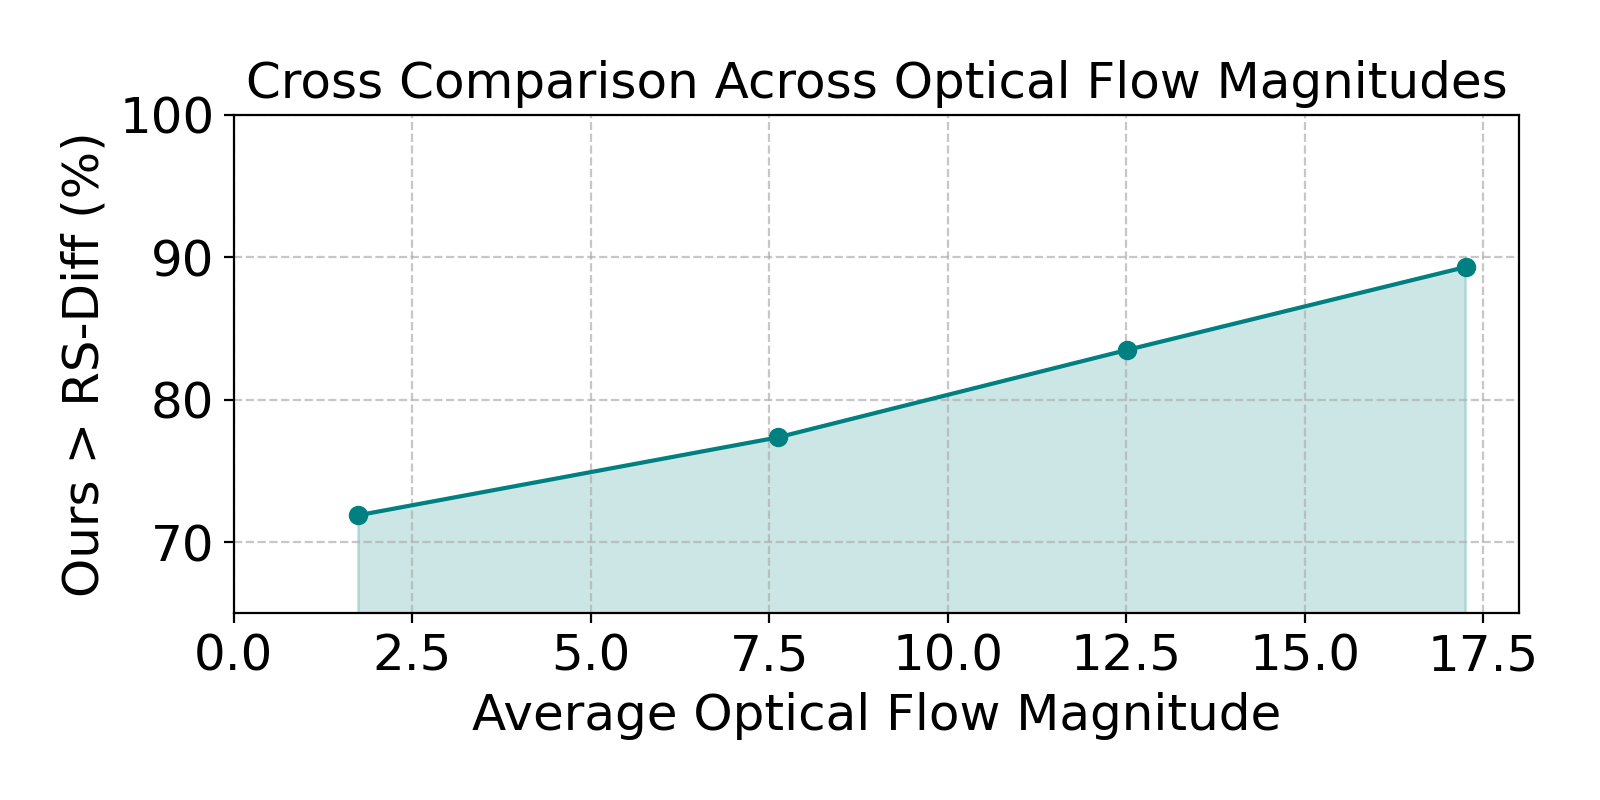
\includegraphics[width=0.9\columnwidth, trim={0cm 0.5cm 0cm 1.5cm}]{collage/psnr_bin_line_vs_flow_zoomed.png}%
    % \vspace{-2mm}
    \caption{Relative performance of our model vs. RS-Diffusion across optical flow magnitudes. Each bin represents the percentage of images where our model achieves higher PSNR.}
    \label{fig:flow_vs_perf}
    \vspace{-1mm}
\end{figure}


\begin{figure}[b!]
    \vspace{-3mm}
    \centering
    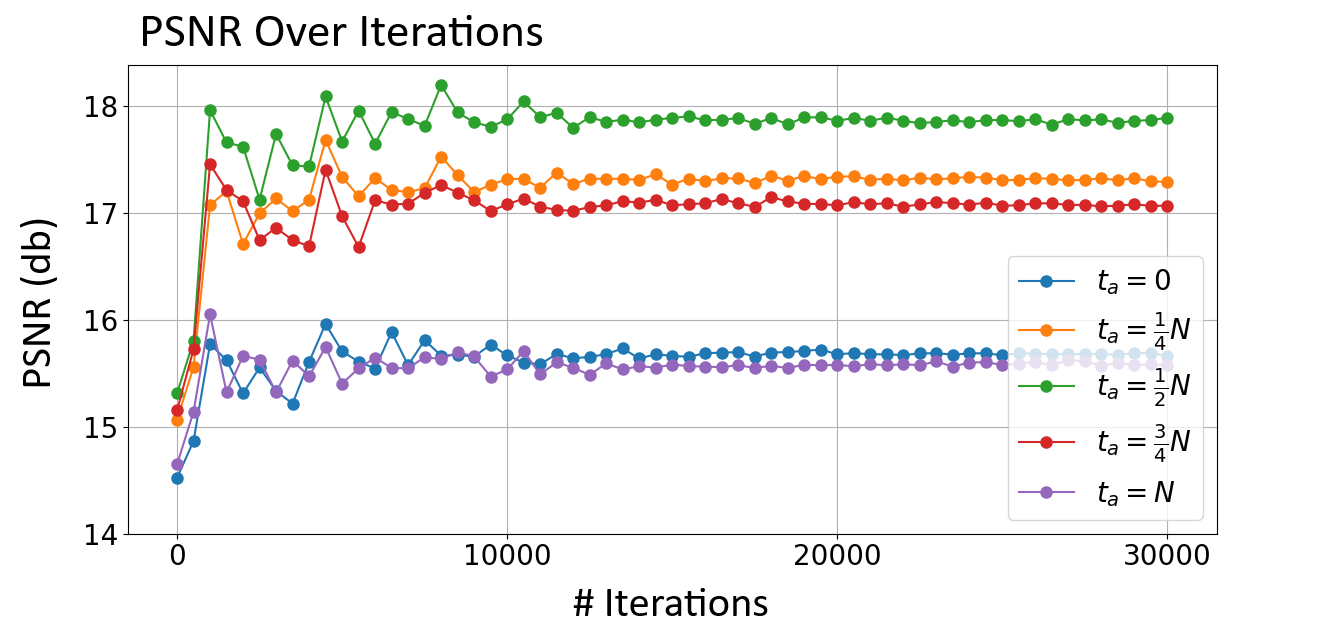
\includegraphics[width=0.49\textwidth, trim=0 2 0 16.5mm,  % left bottom right top
        clip]{X4K_data/figure (1).png} % Path to your first image
    
    \caption{Comparison of PSNR in the five models described in Sec. V-B. Performing a grid search on the possible anchor point location yielded different networks with varying accuracies. These experiments support the use of the anchor point $\frac{N}{2}$ for the real-world scenes.}

    % Comparison of PSNR in the five models described in Sect. 5.B. Each model, with a different anchor point, is represented by a different color on the graph. We validated our theory for anchor points for general scenes. Performing a grid search on the possible anchor point location yielded different networks with varying accuracies. This experiments supported the use of the anchor point $\frac{N}{2}$ for the real-world scenes.
    \vspace{-2mm}
    \label{fig:PSNR_X4K}
\end{figure}









\begin{table}[t!]
\vspace{1mm}
  \caption{Comparisons of anchor points with the first stage of our architecture on \textbf{SYN2} and \textbf{REAL}. These comparisons were conducted on the intermediate RGB images, and $t_a = \frac{N}{2}$ consistently achieves the best or comparable performance.}
  \centering
  \begin{tabular}{c c c c c}
    \hline
    \multirow{2}{*}{Anchor} & \multicolumn{2}{c}{X4K} & \multicolumn{2}{c}{Collocated} \\
    & PSNR & SSIM & PSNR & SSIM \\
    \hline
    $t_a=0$ & 15.594 & 0.578 & 20.238 & 0.639 \\
    $t_a=\frac{N}{4}$ & 17.291 & \textbf{0.630} & 20.292 & 0.640 \\
    $t_a=\frac{N}{2}$ & \textbf{17.733} & 0.629 & \textbf{21.778} & \textbf{0.674} \\
    \hline
  \end{tabular}
  \label{table:AnchorPoint_multi}
  \vspace{-4mm}
\end{table}




\subsection{Ablation Study: Model Configuration}
We evaluated three configurations: \textbf{one-stage}, \textbf{parallel two-stage}, and \textbf{orthogonal two-stage} (Table~\ref{table:collocated_orthogonal_table}). 
\textbf{One-stage} models (Marigold~\cite{StableDiffusion}, Depth-Anything~\cite{DepthAnything}, EcoDepth~\cite{ecodepth}) jointly learn de-rolling and depth but struggle with structural consistency. \textbf{Parallel two-stage} models decouple the tasks sequentially using identical architectures; this improves stability but provides limited gains. 
\textbf{Orthogonal two-stage} models combine distinct architectures (Marigold U-Net for de-rolling and Depth-Anything-V2 for depth) and achieve the highest PSNR, SSIM, AbsRel, and $\delta_1$. Even untuned orthogonal baselines outperform parallel two-stage designs, indicating that sequential specialization of tasks is a pivotal factor behind performance improvements. Fine-tuning further improves results, confirming that the pipeline effectively leverages VFMs for RSC and Monocular Depth Estimation.

\draft{The effects of anchor-point selection and architecture choice were studied independently. Table II isolates anchor-point selection while holding the underlying network architecture fixed. Table III evaluates different architectural configurations while using the optimal anchor point identified in Table II. The results indicate that both factors contribute to performance. Anchor-point selection consistently improves photometric reconstruction quality, while architectural specialization further improves downstream depth estimation metrics.}

% \draft{Because depth estimation is applied to the output of the RS correction stage, and because improvements in PSNR/SSIM consistently correlated with improvements in AbsRel and $\delta1$ throughout our experiments, we performed anchor-point ablations using the intermediate RGB reconstruction metrics. This isolates the effect of anchor-point selection while avoiding confounding effects from retraining multiple downstream depth networks.}


\subsection{Ablation Study: Anchor Points in Other RSC Algorithms}
We evaluated RS-Diffusion~\cite{RS-Diffusion} across a sweep of anchor points and found that centering the predicted flow at the temporal midpoint ($t_{\text{anch}} = \frac{N}{2}$) consistently yields the best reconstruction on synthetic and real RS images. \draft{RS-Diffusion was chosen for ablation due to its ability to change predicted flow easily without retraining.} This confirms that mid-exposure alignment improves performance across different RSC methods without retraining, highlighting the generality of the anchor-point insight (Fig. \ref{fig:teaser_results}).



\begin{table}[t!]
    \centering
    \caption{Depth estimation performance in a legged robot scenario comparing the rolling shutter depth against our method. AbsRel and $\delta_1$ are averaged over $1500$ images collected across three outdoor locations.}
    \setlength{\tabcolsep}{12pt}
    \renewcommand{\arraystretch}{1.2}
    \begin{tabular}{lcc}
        \toprule
        Method & absRel $\downarrow$ & $\delta_1 \uparrow$ \\
        \midrule
        Raw RS Image & 0.112 & 0.895 \\
        Our Algorithm & \textbf{0.096} & \textbf{0.903} \\
        \bottomrule
    \end{tabular}

    \label{tab:puppy_pi}
\end{table}




\subsection{Effectiveness on Legged Robots}

% Legged robots are subject to rapid and irregular motion. Because RS cameras expose image rows sequentially, abrupt accelerations and rotations induce geometric warping that degrades depth estimation. As shown in Fig.~\ref{Fig:puppy_pi_qual}, the RS depth maps exhibit visible distortions that can negatively impact downstream perception and planning.

To evaluate our method in this real-world setting, we collected $1500$ images across three outdoor locations using the collocated sensor system mounted on Puppy-Pi. Runtime measurements were performed on an NVIDIA RTX A6000 GPU using FP16 inference at a resolution of $300\times300$. To improve deployment efficiency, the diffusion model was accelerated by reducing the number of denoising steps from $50$ to $10$, reducing the average inference time from $2850$~ms to $349$~ms.

As shown in Table~\ref{tab:puppy_pi}, our method reduces AbsRel by $14.3\%$ and improves $\delta_1$ accuracy by $0.9\%$ over raw RS input without additional fine-tuning beyond training on the REAL dataset. The qualitative results in Fig.~\ref{Fig:puppy_pi_qual} are consistent with these improvements, where rolling shutter--induced warping is visibly mitigated. While the proposed pipeline demonstrates promising low-latency performance, deployment at higher image resolutions or alongside additional perception tasks presents a natural computational trade-off due to increased diffusion and image-processing costs. Improving scalability through more efficient diffusion strategies, model compression, or shared-backbone architectures remains an important direction for future work.

% \begin{figure}[h!]
%     \centering

%     % =======================
%     % Top row: diagram + single example column
%     % =======================
%     \begin{minipage}{0.95\linewidth}
%         \centering
%         % Combined diagram and example
%         \begin{minipage}{0.5\linewidth}
%             \centering
%             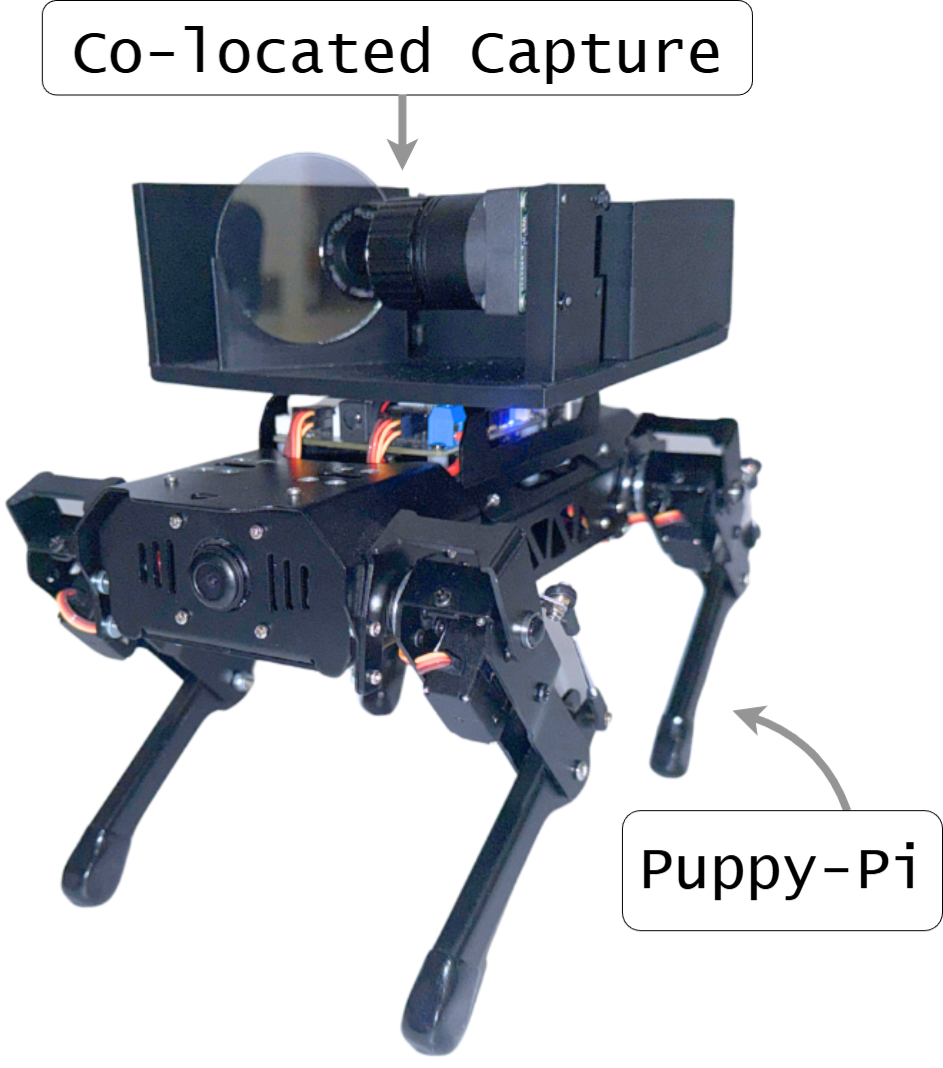
\includegraphics[width=\linewidth]{Figures/puppy-pi.drawio.png}
%         \end{minipage}%
%         \hspace{1mm}
%         \begin{minipage}{0.25\linewidth}
%             \centering
%             % Example column: Input / Prediction / Ground Truth
%             % Row 1 — Input
%             \begin{minipage}{0.2\linewidth}
%                 \centering
%                 \rotatebox{90}{\small Input}
%             \end{minipage}%
%             \begin{minipage}{0.75\linewidth}
%                 \centering
%                 
\includegraphics[width=\textwidth]{puppy-pi/rs/frame55.png}
%             \end{minipage}

%             \vspace{1mm}

%             % Row 2 — Prediction
%             \begin{minipage}{0.2\linewidth}
%                 \centering
%                 \rotatebox{90}{\small Prediction}
%             \end{minipage}%
%             \begin{minipage}{0.75\linewidth}
%                 \centering
%                 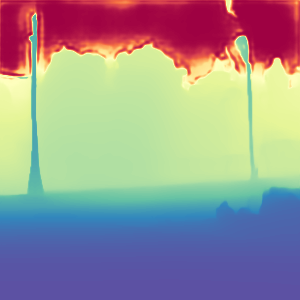
\includegraphics[width=\textwidth]{puppy-pi/depth/rs/frame55_pred.png}
%             \end{minipage}

%             \vspace{1mm}

%             % Row 3 — Ground Truth
%             \begin{minipage}{0.2\linewidth}
%                 \centering
%                 \rotatebox{90}{\small Ground Truth}
%             \end{minipage}%
%             \begin{minipage}{0.75\linewidth}
%                 \centering
%                 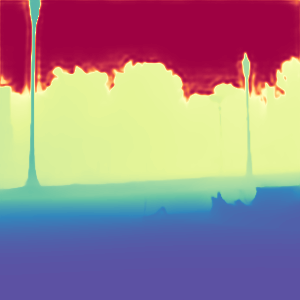
\includegraphics[width=\textwidth]{puppy-pi/depth/gs/frame55.png}
%             \end{minipage}
%         \end{minipage}
%     \end{minipage}

%     \vspace{2mm}

%     % =======================
%     % Bottom: Table
%     % =======================
%     \begin{minipage}{0.65\linewidth}
%         \centering
%         \begin{tabular}{lcc}
%             \toprule
%             Method & absRel $\downarrow$ & $\delta 1 \uparrow$ \\
%             \midrule
%             Raw RS Image & 0.1119 & 0.8958 \\
%             Our Algorithm & \textbf{0.0963} & \textbf{0.9033} \\
%             \bottomrule
%         \end{tabular}
%     \end{minipage}

%     \caption{Left: schematic illustration of the RS effect on the Puppy-Pi. Right: input, prediction, and ground truth for a single frame. Bottom: dataset-averaged depth metrics comparing raw RS input and corrected output. 
%     %\JI{What does this image/result mean...please revise @Vaishnav }
%     }
%     \label{fig:puppy}
% \end{figure}

\begin{figure}[t]
\centering
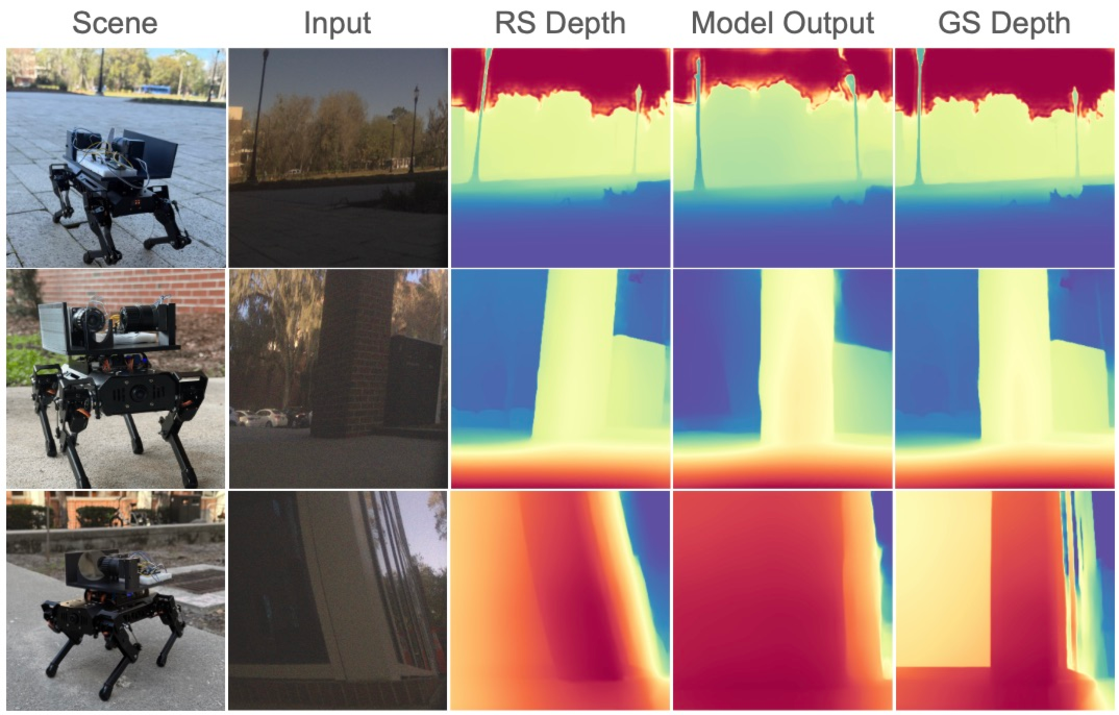
\includegraphics[width=0.49\textwidth]{Figures/puppy_pi_exp_short.pdf}
\caption{Visualizations of our model for RS distortions in legged robots. The qualitative results demonstrate effective rectification of rolling shutter artifacts in legged robotic scenarios.}
\label{Fig:puppy_pi_qual}
\vspace{-3mm}
\end{figure}

%mention number of images/ Scene where rolling shutter is more pronounced, Add rolling shutter output in  image.
% To validate the applicability of our method to mobile robotics, a test dataset was captured with the co-located system attached to Puppy-Pi. The model, using the same weights as the one trained on the co-located dataset, was modified through floating-point changes (32 to 16) and denoise steps (50 to 10) to drastically reduce runtime. These changes reduce average runtime on the pipeline from 2850ms to 349ms, providing a close to real time pipeline for inference. Highlighted visualizations and metrics from data captured on puppy-pi and model output can be seen in Fig. \ref{fig:puppy}.
% \subsection{Ablation Study: Anchor Points}

% Finally, we evaluated the impact of anchor points across synthetic (\textbf{SYN2}) and real-world (\textbf{REAL}) datasets. For SYN2, we trained models with anchor points $t_a = 0, \frac{1}{4}N, \frac{1}{2}N, \frac{3}{4}N, N$, using identical RS inputs. PSNR and SSIM consistently improved as the anchor approached the midpoint, confirming the theoretical prediction (Fig.~\ref{fig:PSNR_X4K}).  

% In REAL, each anchor corresponds to a distinct capture, introducing natural variation. Models trained near the temporal midpoint again achieved higher PSNR and SSIM, demonstrating that the anchor-point formulation generalizes to real-world scenes. These results emphasize the importance of temporal alignment in RS-GS correction, independent of the specific architectures used.

% \noindent \textbf{Effect of Anchor Point on RS-Diffusion.} 


%\JI{What did we learn and where are the closing paragraph}


% \JI{Missing conclusion section}